\documentclass[letterpaper,10pt,twocolumn,titlepage]{article}

\usepackage{graphicx}
\usepackage{amssymb}
\usepackage{amsmath}
\usepackage{amsthm}

\usepackage{alltt}
\usepackage{float}
\usepackage{color}
\usepackage{url}

\usepackage{balance}
\usepackage[TABBOTCAP, tight]{subfigure}
\usepackage{enumitem}
\usepackage{pstricks, pst-node}


\usepackage{geometry}
\geometry{textheight=8.5in, textwidth=6in}

%random comment

\newcommand{\cred}[1]{{\color{red}#1}}
\newcommand{\cblue}[1]{{\color{blue}#1}}

\usepackage{hyperref}
\usepackage{geometry}

\def\name{Xinyue Lu}

%% The following metadata will show up in the PDF properties
\hypersetup{
  colorlinks = true,
  urlcolor = black,
  pdfauthor = {\name},
  pdfkeywords = {cs311 ``operating systems'' files filesystem I/O},
  pdftitle = {CS 311 Project 1: UNIX File I/O},
  pdfsubject = {CS 311 Project 1},
  pdfpagemode = UseNone
}

\begin{document}

Running time according to chunk size

\begin{table}[!htp]
    \begin{tabular}{|l|l|}
        \hline
        Chunk Size & Running Time (in ms) \\ \hline
        1 & 49753713 \\ \hline
        2 & 25116569 \\ \hline
        4 & 13956130 \\ \hline
        8 & 6323719 \\ \hline
        16 & 3177433 \\ \hline
        32 & 1606840 \\ \hline
        64 & 823184 \\ \hline
        128 & 429793 \\ \hline
        256 & 237527 \\ \hline
        512 & 138264 \\ \hline
        1024 & 96577 \\ \hline
        2048 & 71303 \\ \hline
        4096 & 68371 \\ \hline
        8192 & 60321 \\
        \hline
    \end{tabular}
\end{table}

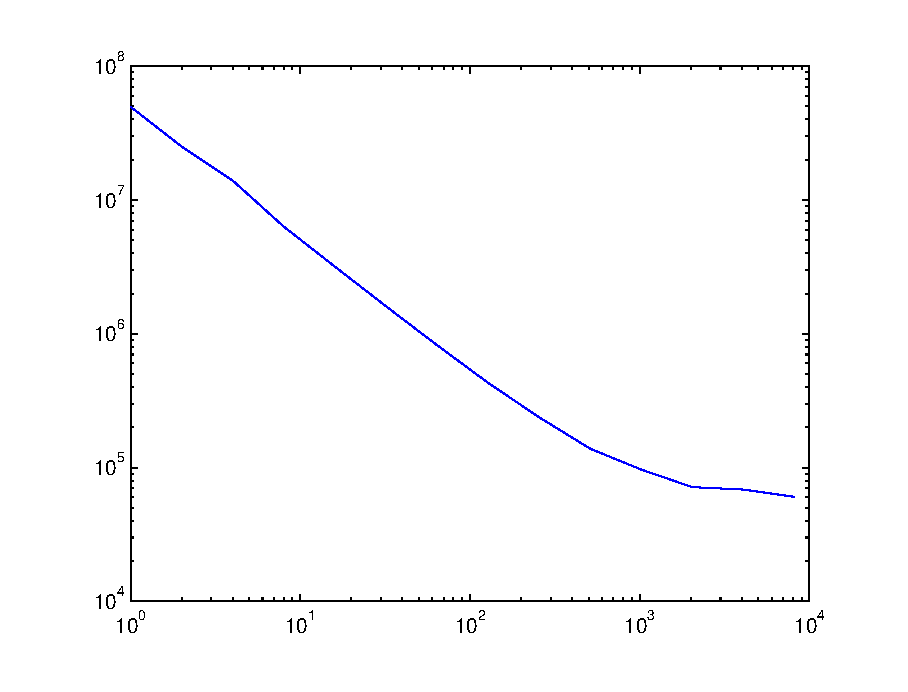
\includegraphics [width=0.6\textwidth]{cs311_1.eps}

Both axis are in log scale.

\end{document}

